\section{Implementation}
\begin{frame}{Implementation}
    \begin{itemize}
        \item Data Collection \& Preprocessing
        \item Data Augmentation
        \item Classification Model
        \item Virtual Environment
    \end{itemize}
\end{frame}

\subsection*{Data Collection \& Preprocessing}
\begin{frame}{Data Collection \& Preprocessing}
    \begin{minipage}[c]{.6\textwidth}
        \begin{itemize}
            \item Datasets: Physionet, Weibo, BCI Competition IV
            \item Channels: 58
            \item Frequency Bandpass Filter: 0.5~\textemdash{}~40 Hz
            \item Start-End Window Time: 0.0~\textemdash{}~0.5 s
            \item Sampling Frequency: 128 Hz
        \end{itemize}
    \end{minipage}
    \begin{minipage}[c]{.39\textwidth}
        \begin{figure}[!htbp]
            \centering
            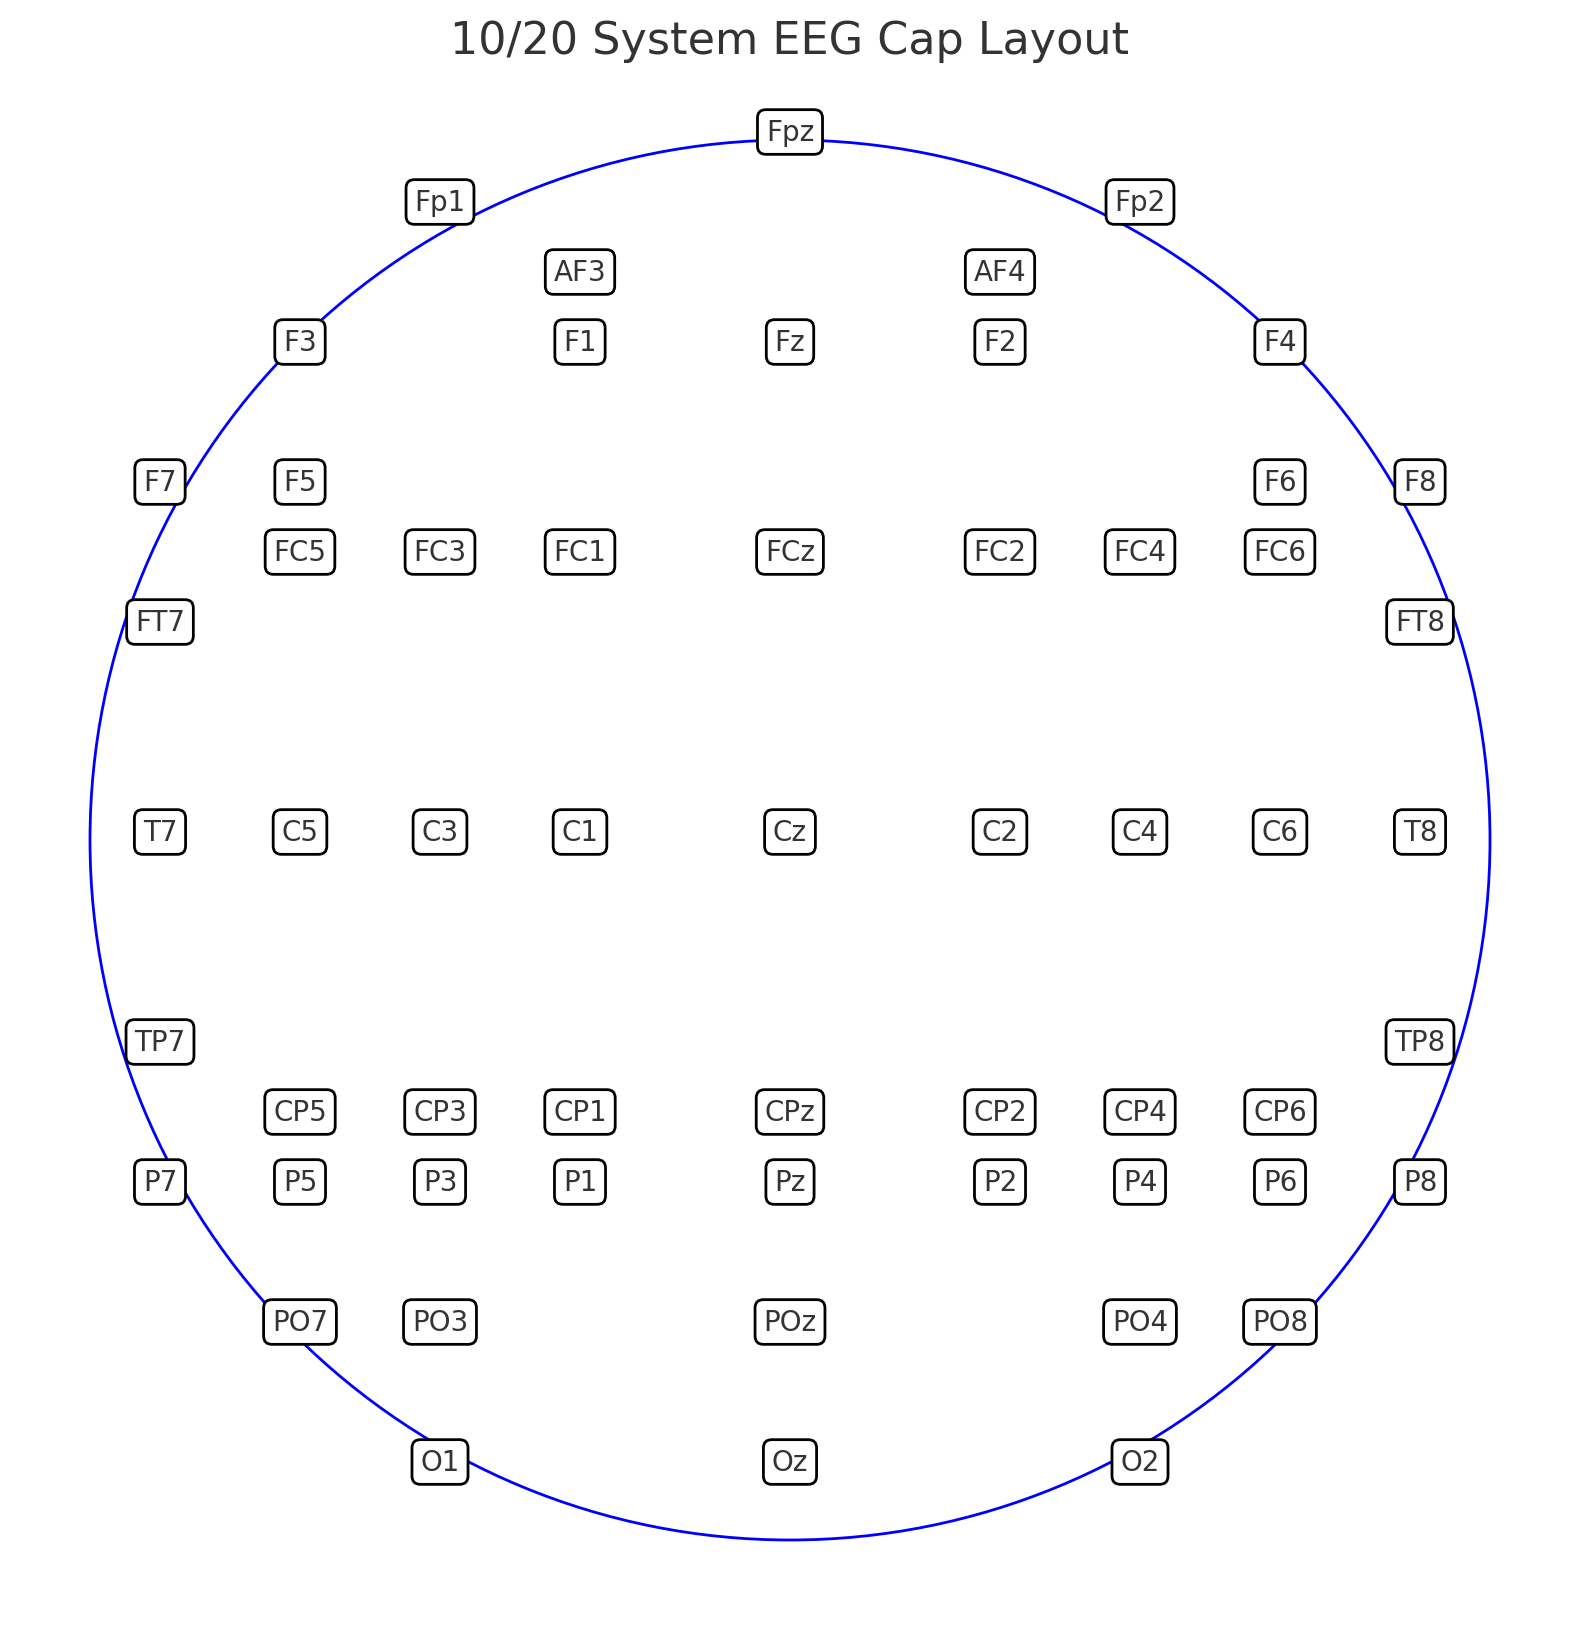
\includegraphics[width=0.5\textwidth]{figures/Methodology/thesis_eeg_cap}
        \end{figure}
    \end{minipage}
\end{frame}

\subsection*{Data Augmentation}
\begin{frame}{Data Augmentation}
    \begin{itemize}
        \item Stochastic Noise Injection
        \item Generative Adversarial Networks (GANs)
    \end{itemize}
\end{frame}
\begin{frame}{Data Augmentation \textemdash{} Noise Injection}
    \begin{itemize}
        \item Reduced Dataset size
        \item Gaussian Noise
        \begin{itemize}
            \item Mean: 0.0
            \item Standard Deviation: 1.0
        \end{itemize}
    \end{itemize}
\end{frame}
\begin{frame}{Data Augmentation \textemdash{} GANs}
    \begin{minipage}[c]{.6\textwidth}
        \begin{itemize}
            \item Loss Function: Binary Cross-Entropy
            \item Optimizer: Adam
            \item Learning Rate: 0.0002
            \item Train Epochs: 100 epochs, with changing number of steps
        \end{itemize}
    \end{minipage}
    \begin{minipage}[c]{.39\textwidth}
        \begin{figure}[!htbp]
            \centering
            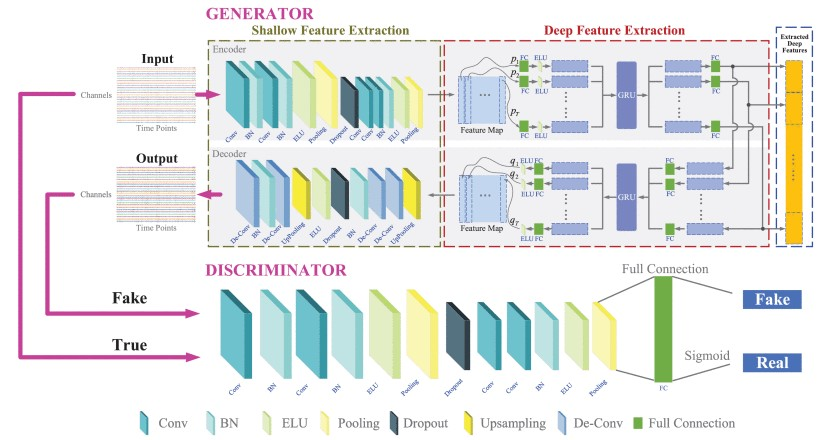
\includegraphics[width=\textwidth]{figures/Methodology/GAN}
        \end{figure}
    \end{minipage}
\end{frame}

\subsection*{Classification Model}
\begin{frame}{Classification Model}
    \begin{itemize}
        \item Long Short-Term Memory (LSTM)
        \item Attention Mechanism
    \end{itemize}
\end{frame}
\begin{frame}{Classification Model \textemdash{} LSTM}
    \begin{minipage}[c]{.6\textwidth}
        \begin{itemize}
            \item Hidden Units: 100 + 50
            \item Activation Function: Softmax
            \item Optimizer: Adam
            \item Learning Rate: 0.01
            \item Loss Function: Categorical Cross Entropy
        \end{itemize}
    \end{minipage}
    \begin{minipage}[c]{.39\textwidth}
        \begin{figure}[!htbp]
            \centering
            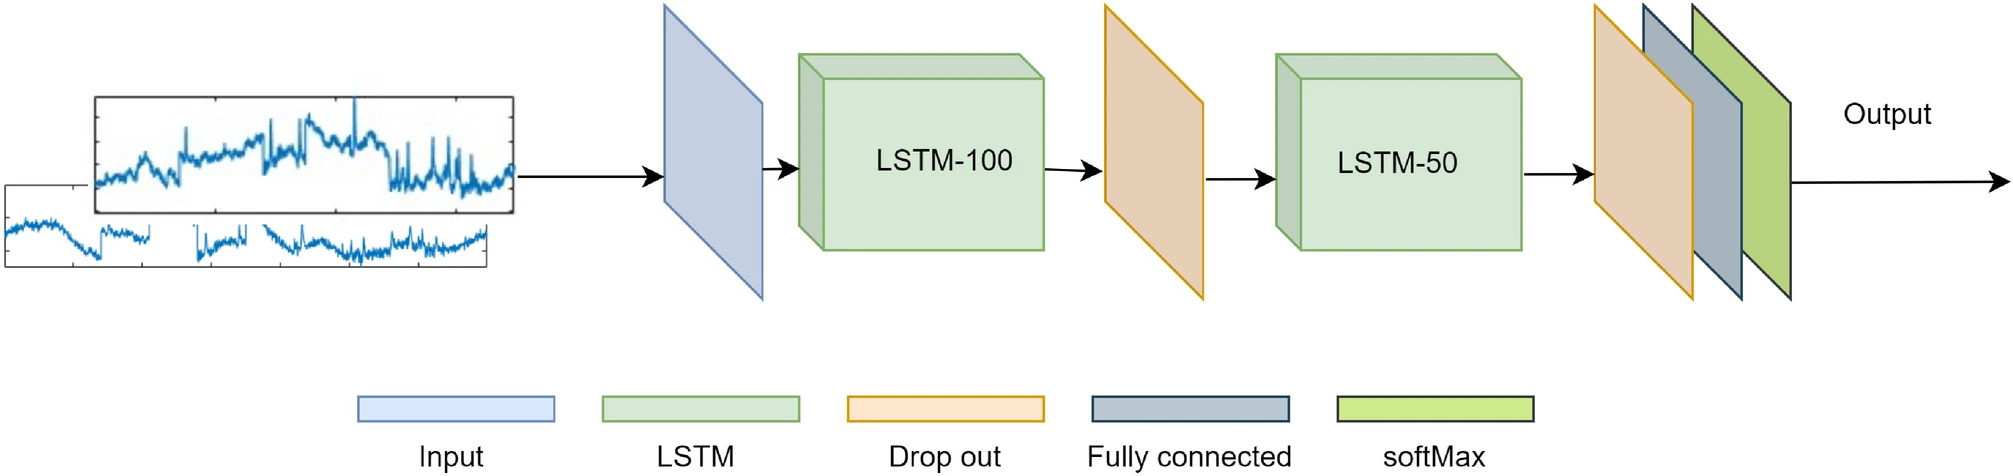
\includegraphics[width=\textwidth]{figures/Methodology/LSTM}
        \end{figure}
    \end{minipage}
\end{frame}
\begin{frame}{Classification Model \textemdash{} Attention Mechanism}
    \begin{minipage}[c]{.6\textwidth}
        \begin{itemize}
            \item Number of Layers: 4 Attention Layers
            \item Activation Function: Softmax
            \item Optimizer: Adam
            \item Learning Rate: 0.01
            \item Loss Function: Categorical Cross Entropy
        \end{itemize}
    \end{minipage}
    \begin{minipage}[c]{.39\textwidth}
        \begin{figure}[!htbp]
            \centering
            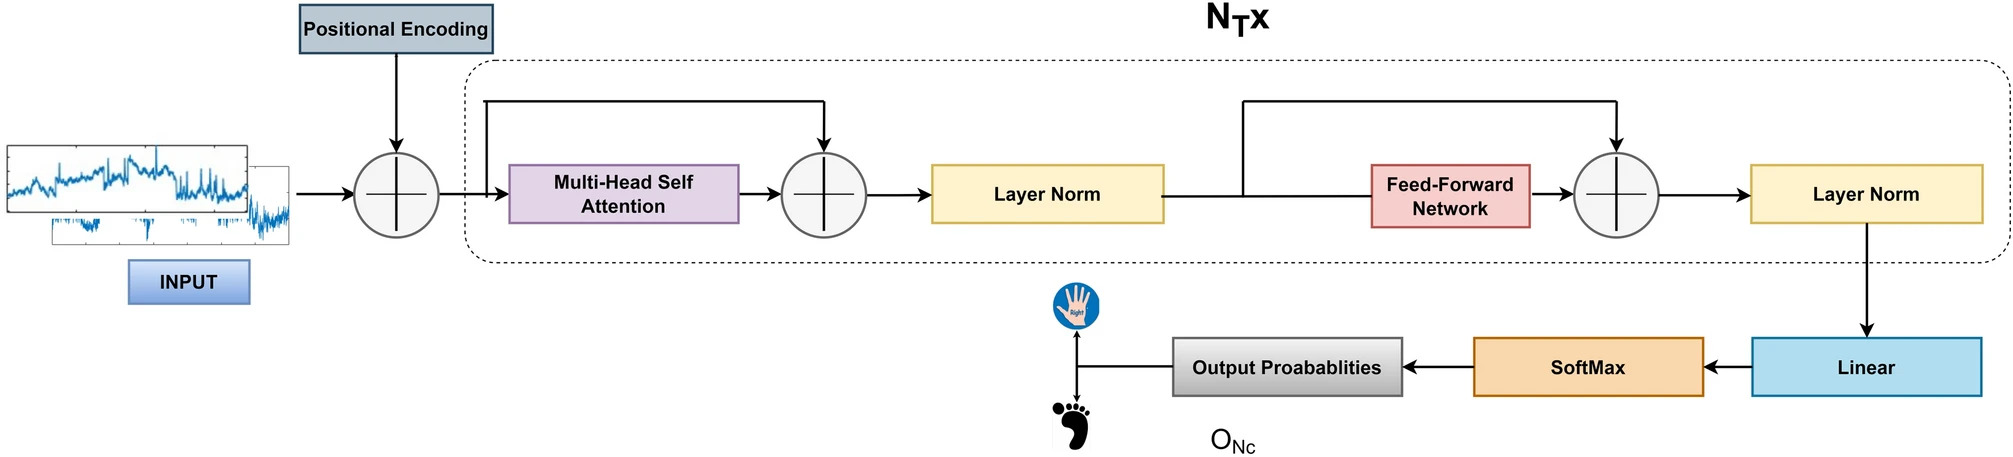
\includegraphics[width=\textwidth]{figures/Methodology/Attention}
        \end{figure}
    \end{minipage}
\end{frame}

\subsection*{Virtual Environment}
\begin{frame}{Virtual Environment}
    \begin{minipage}[c]{.5\textwidth}
        \begin{itemize}
            \item TextMeshPro
            \item Starter Assets \textemdash{} Third Person Controller
            \item Native Websocket $\xrightarrow{}$ Open source library
            \item Unity AI Navigation
            \item Maze Generator $\xrightarrow{}$ Free Unity Asset
        \end{itemize}
        \begin{figure}[!htbp]
            \centering
            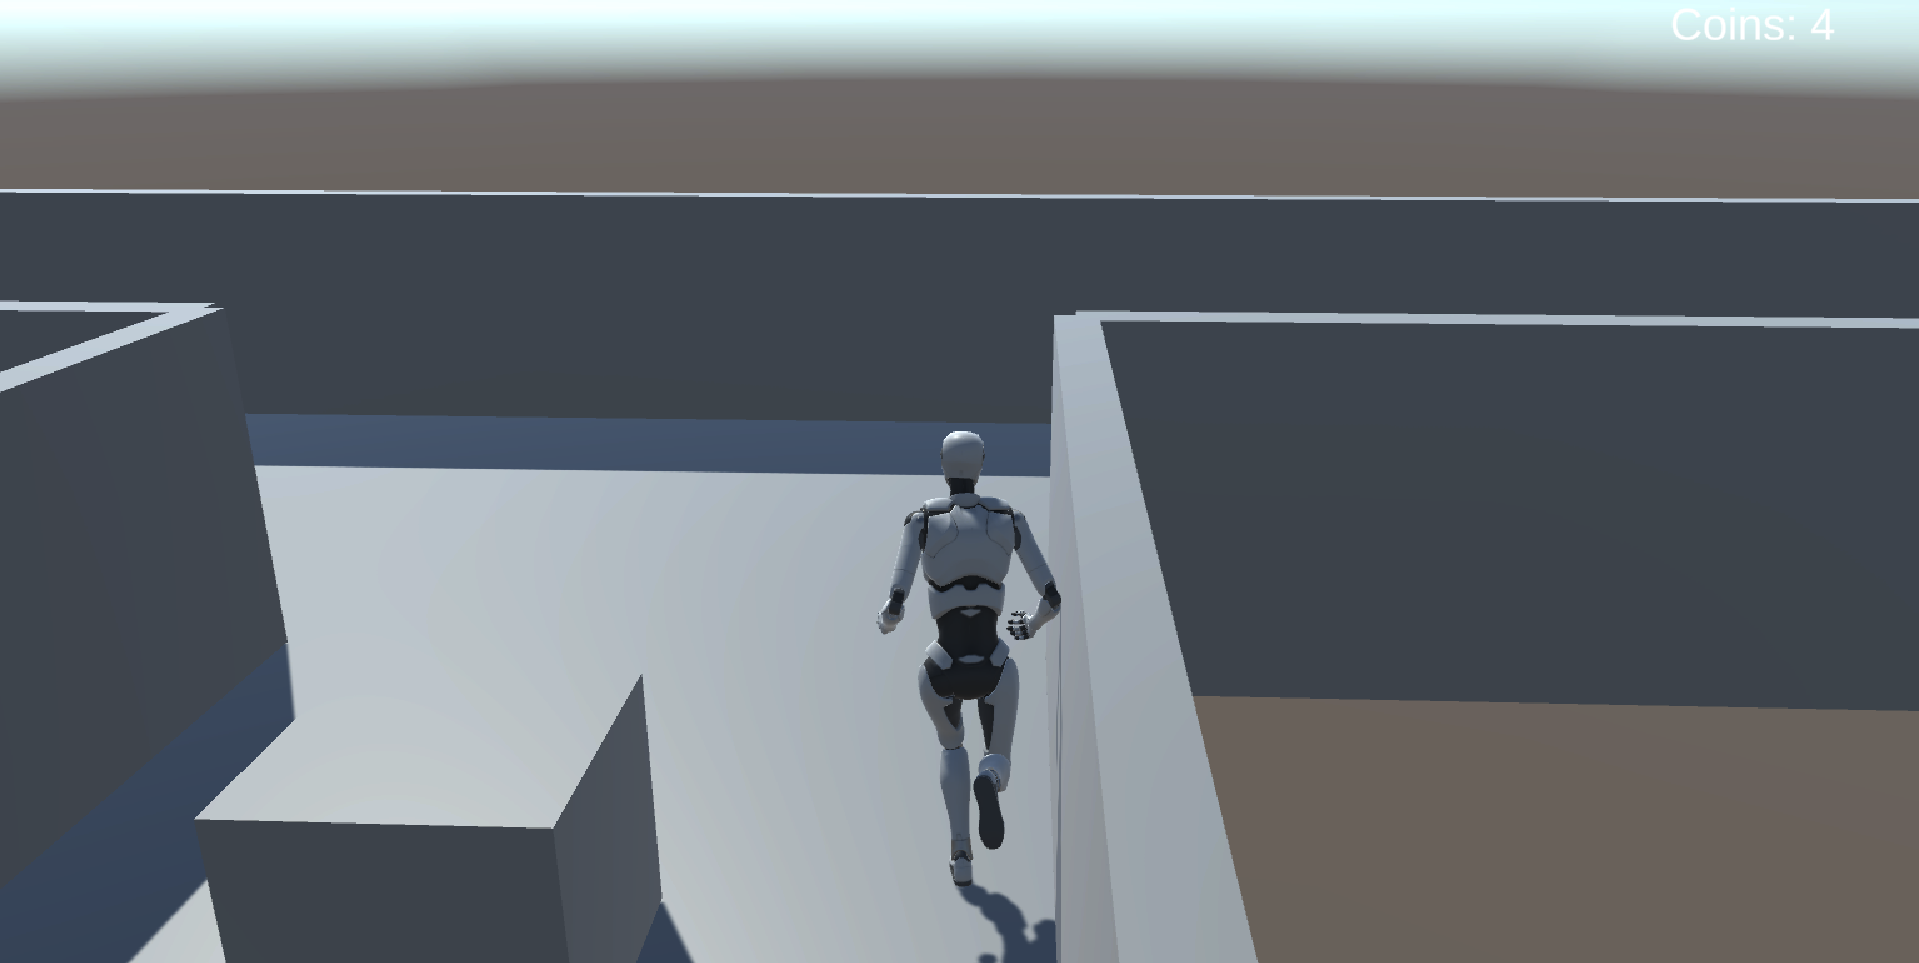
\includegraphics[width=.49\textwidth]{figures/Methodology/infinite_runner}
            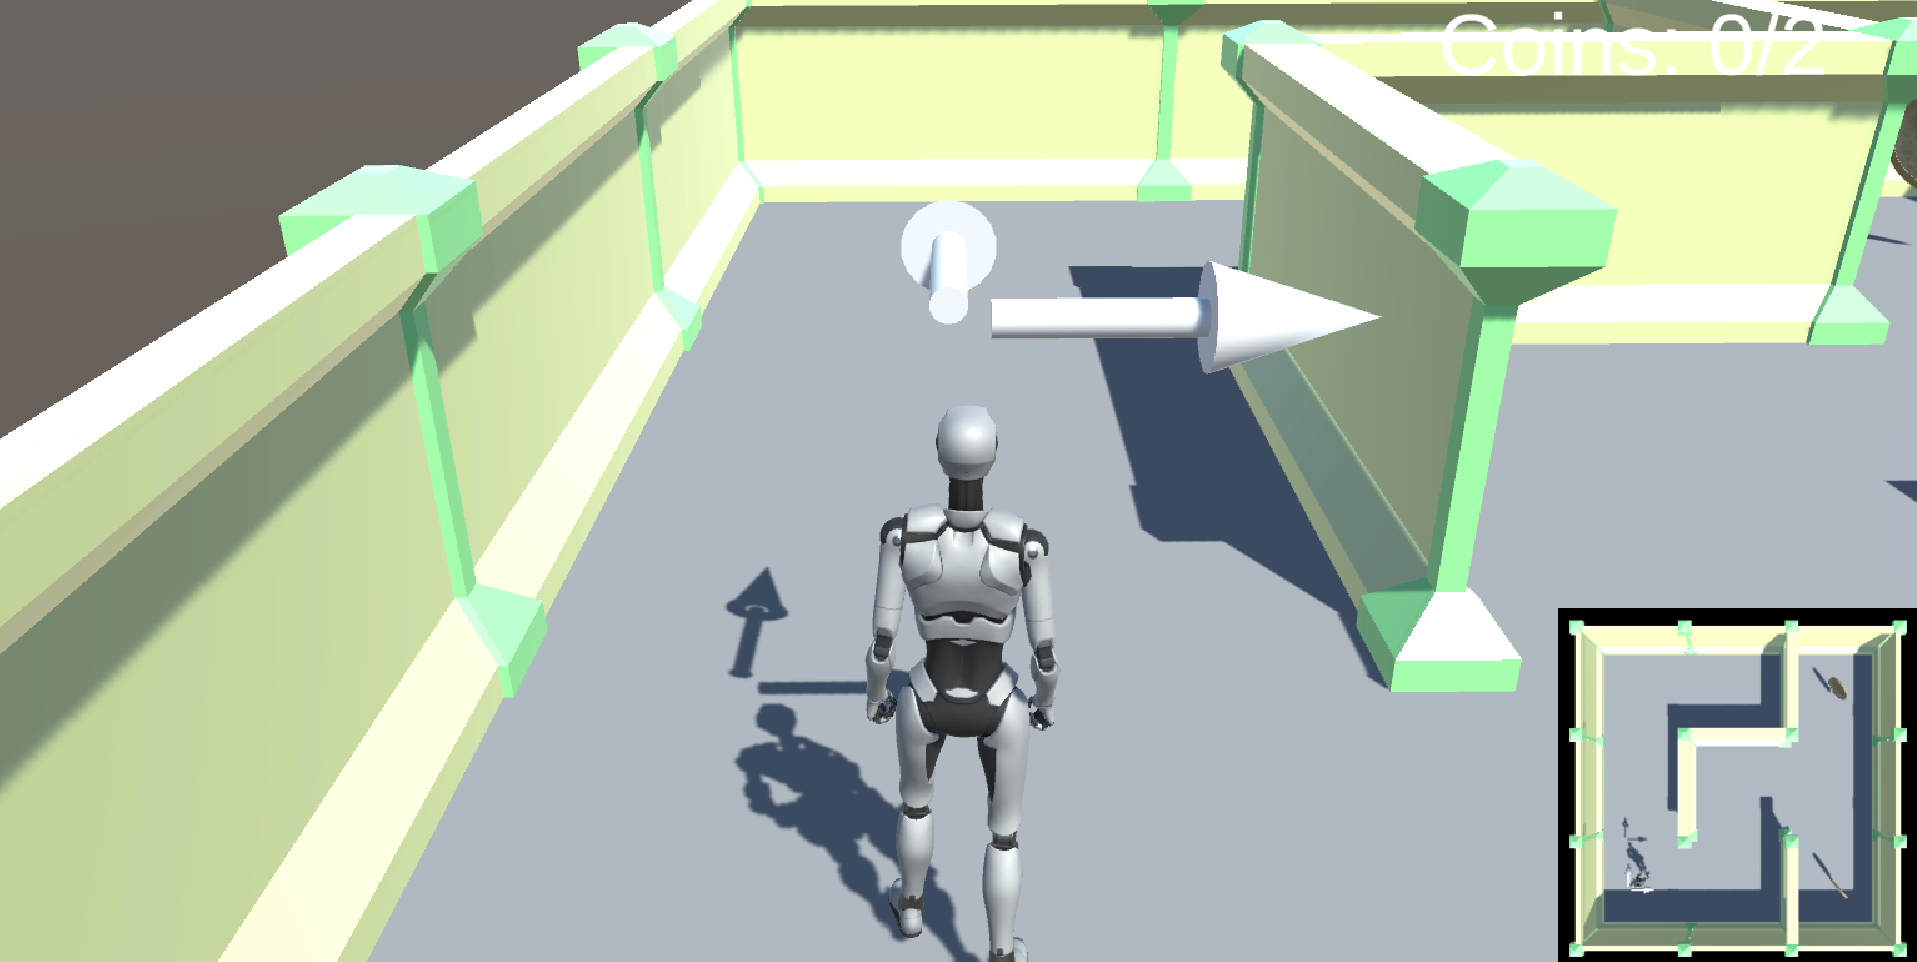
\includegraphics[width=.49\textwidth]{figures/Methodology/maze}
        \end{figure}
    \end{minipage}
    \begin{minipage}[c]{.49\textwidth}
        \begin{figure}[!htbp]
            \centering
            \scalebox{0.25}{
                \begin{tikzpicture}[
                    squarednode/.style={rectangle, draw=black, very thick, minimum size=5mm},
                    diamondnode/.style={diamond, draw=black, very thick},
                    ]
                    %Nodes
                    \node[squarednode] (player) {Player Walks};
                    \node[squarednode, below=of player] (rotate) {Eventually Rotate Player and Camera};
                    \node[squarednode, below=of rotate] (delete) {Delete Not Visible Tiles};
                    \node[squarednode, below=of delete, dashed] (generate) {Generate New Tiles};
                    \node[diamondnode, below=of generate] (hasleft) {Has Left Tile};
                    \node[squarednode, below right=of hasleft] (generateleft) {Generate Left Tile};
                    \node[diamondnode, below=of hasleft] (hasright) {Has Right Tile};
                    \node[squarednode, below right=of hasright] (generateright) {Generate Right Tile};
                    \node[diamondnode, below=of hasright] (hasforward) {Has Forward Tile};
                    \node[squarednode, below right=of hasforward] (generateforward) {Generate Forward Tile};
                    \node[squarednode, below=of hasforward] (foreach) {Foreach Next Tile};
                    \node[diamondnode, below=of foreach] (hasobstacle) {Has Obstacle};
                    \node[squarednode, below right=of hasobstacle] (generateobstacle) {Generate Obstacle};
                    \node[squarednode, below=of hasobstacle] (deletewall) {Delete Wall};
                    \node[squarednode, below=of deletewall] (tilegenerated) {Tile Generated};
                    %Lines
                    \draw[->] (player) -- node[right] {Cross end of path collider} (rotate);
                    \draw[->] (rotate) -- (delete);
                    \draw[->] (delete) -- (generate);
                    \draw[->] (generate) -- (hasleft);
                    \draw[->] (hasleft) -- node[right] {No} (hasright);
                    \draw[->] (hasleft) -- node[right] {Yes} (generateleft);
                    \draw[->] (generateleft) -- (hasright);
                    \draw[->] (hasright) -- node[right] {No} (hasforward);
                    \draw[->] (hasright) -- node[right] {Yes} (generateright);
                    \draw[->] (generateright) -- (hasforward);
                    \draw[->] (hasforward) -- node[right] {No} (foreach);
                    \draw[->] (hasforward) -- node[right] {Yes} (generateforward);
                    \draw[->] (generateforward) -- (foreach);
                    \draw[->] (foreach) -- (hasobstacle);
                    \draw[->] (hasobstacle) -- node[right] {Yes} (generateobstacle);
                    \draw[->] (hasobstacle) -- node[right] {No} (deletewall);
                    \draw[->] (deletewall) -- (tilegenerated);
                    \draw[->] (generateobstacle) -- (deletewall);
                    \draw[->] (tilegenerated) to[out=180, in=180] (foreach);
                \end{tikzpicture}
            }
        \end{figure}
    \end{minipage}
\end{frame}
